% Created 2019-04-30 Tue 19:50
% Intended LaTeX compiler: pdflatex
\documentclass[11pt]{article}
\usepackage[utf8]{inputenc}
\usepackage[T1]{fontenc}
\usepackage{graphicx}
\usepackage{grffile}
\usepackage{longtable}
\usepackage{wrapfig}
\usepackage{rotating}
\usepackage[normalem]{ulem}
\usepackage{amsmath}
\usepackage{textcomp}
\usepackage{amssymb}
\usepackage{capt-of}
\usepackage{hyperref}
\author{Heitor Lourenço Werneck \\{\href{mailto:heitorwerneck@hotmail.com}{heitorwerneck@hotmail.com}}}
\usepackage[portuguese]{babel}
\usepackage{amsmath}
\usepackage[binary-units=true]{siunitx}
\usepackage[top=0.5cm,bottom=1.2cm,left=2cm,right=2cm]{geometry}
\usepackage{mdframed}
\usepackage{algorithm}
\usepackage{listings}
\usepackage{algpseudocode}
\usepackage{tikz}
\usetikzlibrary{shapes,arrows}
\usepackage{mathtools}
\date{\today}
\title{Algoritmos e Estrutura de Dados III (2019-1)\\\medskip
\large Trabalho Prático 1}
\hypersetup{
 pdfauthor={Heitor Lourenço Werneck},
 pdftitle={Algoritmos e Estrutura de Dados III (2019-1)},
 pdfkeywords={},
 pdfsubject={},
 pdfcreator={Emacs 26.1 (Org mode 9.2.2)}, 
 pdflang={Portuguese}}
\begin{document}

\maketitle
\tableofcontents

\definecolor{bg}{rgb}{0.95,0.95,0.95}
\BeforeBeginEnvironment{minted}{\begin{mdframed}[backgroundcolor=bg]}
\AfterEndEnvironment{minted}{\end{mdframed}}
\numberwithin{equation}{section}
\algnewcommand{\IfThenElse}[3]{% \IfThenElse{<if>}{<then>}{<else>}
  \State \algorithmicif\ #1\ \algorithmicthen\ #2\ \algorithmicelse\ #3}

% Define block styles
\tikzstyle{decision} = [diamond, draw, fill=blue!20, 
    text width=4.5em, text badly centered, node distance=3cm, inner sep=0pt]
\tikzstyle{block} = [rectangle, draw, fill=blue!20, 
    text width=5em, text centered, rounded corners, minimum height=4em]
\tikzstyle{line} = [draw, -latex']
\tikzstyle{cloud} = [ellipse, draw, fill=red!20, 
    text width=5em, text centered, rounded corners, minimum height=2em]
%\tikzstyle{cloud} = [draw, ellipse,fill=red!20, node distance=3.5cm,
%    minimum height=2em]


\lstset{
  basicstyle=\ttfamily,
  columns=fullflexible,
  frame=single,
  breaklines=true,
  postbreak=\mbox{\textcolor{red}{$\hookrightarrow$}\space},
}
\newpage
\section{Introdução}
\label{sec:org5f27c3b}
O trabalho a ser apresentado consiste na resolução do problema de planejamento de manobras tendo em vista maximizar a ocupação do estacionamento e minimizar o tempo de espera dos clientes para sair do estacionamento. Como o problema parece ser complexo, inicialmente será abordado uma parte simples da solução. Uma breve descrição do programa:
\begin{itemize}
\item O estacionamento é quadrado e tem dimensões 6 por 6.
\item Os carros não fazem curva.
\item As dimensões são identificadas de X1 a X6 e de Y1 a Y6.
\item O estacionamento comporta dois tipos de veículos: carros e caminhões.
\item Carros têm dimensão 2 por 1 e os caminhões têm dimensão 3 por 1.
\item O objetivo é mover um carro específico, que chamaremos Z para a saída do estacionamento.
\item O programa deve receber como entrada a configuração inicial do estacionamento e um conjunto de manobras.
\item Deve responder se teve sucesso ou não em retirar o carro Z.
\end{itemize}

Entrada do programa:
\begin{itemize}
\item Arquivo de configuração inicial no qual informa os veículos e suas posições. Os veículos podem estar posicionados paralelo ao eixo X ou ao eixo Y. Cada linha informa sobre um veículo: identificador, tamanho, direção e posição.
\item Arquivo de manobras no qual informa os movimentos dos veículos. Cada movimento indica o veículo, a dimensão onde o movimento ocorre e a amplitude do movimento.
\end{itemize}

Erros que devem ser alertados:
\begin{itemize}
\item Alertar para configurações físicas impossíveis (isto é, dois veículos ocupando a mesma posição).
\item Manobras inviáveis (colisões entre veículos e com os muros
\end{itemize}
do estacionamento).

Logo será criado um simulador de um estacionamento simplificado. Para resolver esse problema foi utilizado estruturas de dados com boa complexidade assintótica para casos gerais.

\subsection{Uma visão geral sobre a solução}
\label{sec:org210e665}

\begin{center}
\begin{tikzpicture}[node distance = 2.8cm, auto]
    % Place nodes, main nodes
    \node [block] (argumentos) {Execução do programa};
    \node [block, below of=argumentos] (leituraarg) {Le os argumentos passados e abre os arquivos};
    \node [cloud, left of=leituraarg] (arqentradac) {Arquivo de configuração inicial};
    \node [cloud, right of=leituraarg] (arqentradam) {Arquivo de manobras};
    \node [block, below of=leituraarg,xshift=-2cm] (varini) {Inicializa as variaveis};
    \node [block, below of=varini] (containi) {Começa a contar o tempo};
    \node [block, below of=containi] (estacionamento) {Cria o estacionamento};
    \node [block, below of=estacionamento,xshift=-2cm] (manobras) {Aplica manobras};

    \node [block, below of=manobras,xshift=-2cm] (contapara) {Para de contar o tempo};

    \node [cloud, left of=contapara] (contaimprime) {Imprime o tempo};
    \node [block, below of=contapara] (varfim) {Desaloca variaveis};
    % node erros
    \node [cloud, below of=leituraarg,xshift=2cm] (erro1) {Erro na abertura};

    \node [cloud, below of=estacionamento,xshift=2cm] (erro2) {Erro na configuração do estacionamento};
    \node [cloud, below of=manobras,xshift=2cm] (erro3) {Erro na aplicação das manobras};

    % Draw edges
    \path [line,dashed] (argumentos) -- (leituraarg) node [midway, yshift= -0.1cm ,above] (TextNode) {Argumentos};
    \path [line,dashed] (arqentradac) -- (leituraarg);
    \path [line,dashed] (arqentradam) -- (leituraarg);
    \path [line,dashed] (leituraarg) -- (varini) node [midway, yshift= -0.1cm ,above] (TextNode) {Sucesso};
    \path [line,dashed] (varini) -- (containi);
    \path [line,dashed] (containi) -- (estacionamento);
    \path [line,dashed] (estacionamento) -- (manobras) node [midway, yshift= -0.1cm ,above] (TextNode) {Sucesso};
    \path [line,dashed] (estacionamento) -- (erro2) node [midway, yshift= -0.1cm ,above] (TextNode) {Falha};
    \path [line,dashed] (leituraarg) -- (erro1) node [midway, yshift= -0.1cm ,above] (TextNode) {Falha};
    \path [line,dashed] (manobras) -- (erro3) node [midway, yshift= -0.1cm ,above] (TextNode) {Falha};
    \path [line,dashed] (manobras) -- (contapara) node [midway, yshift= -0.1cm ,above] (TextNode) {Sucesso};
    \path [line,dashed] (erro3) -- (contapara);
    \path [line,dashed] (contapara) -- (contaimprime);
    \path [line,dashed] (contapara) -- (varfim);
    \path [line,dashed] (erro2) to[out=-20,in=-70] (varfim);
\end{tikzpicture}
\end{center}

\newpage
\section{Módulos}
\label{sec:orga92d9c7}
\subsection{Estruturas de dados}
\label{sec:org5b1d6c4}
As estruturas de dados são de extrema importância para resolução do problema, elas irão ter grande peso na complexidade do programa e no seu funcionamento.
\subsubsection{Tabela de dispersão}
\label{sec:org5df7046}
A tabela de dispersão \cite{hashingusp} foi utilizada pois visto que há referencia aos nomes respectivos dos veículos constantemente no arquivo de manobras, logo uma tabela de dispersão comum garante complexidade de tempo sobre as operações de inserção e busca de \(\Theta(1)\) e \(O(n)\)(Ao longo do documento será utilizado espalhamento comum para o espalhamento com complexidade \(O(n)\)). É interessante lembrar que existe o espalhamento perfeito (\emph{perfect hashing}) \cite{cormen09_introd} que também foi implementado nesse trabalho que garante complexidade de tempo \(O(1)\) para operações de inserção e busca, porém a complexidade de espaço no pior caso é \(\Omega(n)\). 

A tabela de dispersão normal utilizou a função de espalhamento modular com sondagem linear.

Na análise de resultados será possível ver quão diferente o espalhamento perfeito pode ser no tempo de execução.

O espalhamento perfeito foi utilizado aproveitando-se do fato que os identificadores dos veículos são caracteres, e existem 256 caracteres diferentes, ou seja um numero fixo de entradas possíveis.

A tabela de dispersão principal contem 16 outras tabelas podendo conter 16 objetos, todas elas não alocadas para uma economia de blocos de caracteres não utilizados. 

\begin{equation}\label{eq:HashSize}
\begin{aligned}
\underbrace{obj.label}_{\parbox{1.75cm}{ Rotulo do objeto}} \in \{x : x \in \mathbb{N} \land (0 \leq x \leq 255)\}\\
ASCII\_SIZE = 256\\
HashSize = \frac{ASCII\_SIZE}{16}\\
HashSize = 16\\
\end{aligned}
\end{equation}

Um detalhe de implementação interessante e que na criação da tabela de dispersão com espalhamento perfeito já é alocado os blocos de caracteres previstos como sendo os mais utilizados, que são os blocos que contem A e Z.

\begin{verbatim}
perf_hash->hashs[hash_division('A',TABLE_SIZE)]= new_hash(TABLE_SIZE);
perf_hash->hashs[hash_division('Z',TABLE_SIZE)]= new_hash(TABLE_SIZE);
\end{verbatim}

\usetikzlibrary{decorations.pathreplacing}
\begin{center}
\begin{tikzpicture}
\node (a) at (0,0){
  \begin{tabular}{ | l | c | c | r |}
    \hline
    $Hash_{1}$ & $Hash_{2}$ & ... & $Hash_{HashSize}$ \\ \hline
  \end{tabular}
};
\node[yshift=0.1cm] (headmain) at (a.north){
Tabela de dispersão perfeita
};
\node[yshift=-2cm,xshift=-7.3cm] (b) at (a.south) 
{

  \begin{tabular}{ | l | c | c | r |}
    \hline
    $Obj_{1}$ & $Obj_{2}$ & ... & $Obj_{HashSize}$  \\ \hline
  \end{tabular}
};

\node[yshift=-2cm,xshift=-1.5cm] (c) at (a.south) 
{

  \begin{tabular}{ | l | c | c | r |}
    \hline

    $Obj_{1}$ & $Obj_{2}$ & ... & $Obj_{HashSize}$  \\ \hline
  \end{tabular}
};

\node[yshift=-2cm,xshift=1.7cm] (d) at (a.south) 
{
...
};

\node[yshift=-2cm,xshift=+5cm] (e) at (a.south) 
{
  \begin{tabular}{ | l | c | c | r |}
    \hline
    $Obj_{1}$ & $Obj_{2}$ & ... & $Obj_{HashSize}$  \\ \hline
  \end{tabular}
};
\draw[decorate,decoration={brace, amplitude=10pt, raise=5pt, mirror}]
  (b.south west) to node[black,midway,below= 15pt] {HashSize-Tabelas de dispersão} (e.south east);
\draw[->,ultra thick](a)--(b);
\draw[->,ultra thick](a)--(c);
\draw[->,ultra thick](a)--(d);
\draw[->,ultra thick](a)--(e);

\end{tikzpicture}
\end{center}

\subsubsection{Mapa de Colisão}
\label{sec:org730ec7b}
O mapa de colisão foi feito para trabalhar com a colisão de maneira que ela fosse um evento ou seja, só é preciso checar caso haja alguma mudança no mapa e só ira checar colisões nas áreas de mudança oque garante uma complexidade assintótica ótima.
Também é importante utilizá-lo para diminuir o tempo de busca pelo carro Z para ser O(1) pois caso não haja mapa de colisão com os identificadores dos veículos no mapa esse tempo de busca seria \(O(n)\) em uma tabela de dispersão não perfeita.

\bigskip
Como definido na introdução o tamanho do mapa em cada dimensão é 6 e há 2 dimensões.

\begin{equation}\label{eq:MapSize}
\begin{aligned}
MapDimensions \coloneqq 2\\
MapSize \coloneqq 6
\end{aligned}
\end{equation}


\begin{verbatim}

Y+---+---+---+---+---+---+
6|   |   |   |   |   |   |
 +---+---+---+---+---+---+
5|   |   |   |   |   |   |
 +---+---+---+---+---+---+
4|   |   |   |   | Z | Z |
 +---+---+---+---+---+---+
3|   |   |   |   |   | A |
 +---+---+---+---+---+---+
2|   |   |   |   |   | A |
 +---+---+---+---+---+---+
1|   |   |   |   |   | A |
 +---+---+---+---+---+---+
   1   2   3   4   5   6 X
      Mapa de colisão
\end{verbatim}

O mapa possui funções para inserir objetos nele e ao mesmo tempo detectar colisões devido a inserções e também possui função de remoção do mapa.

\begin{verbatim}
int collission_map_insert(map coll_map,object* obj);
int collission_map_remove(map coll_map,object* obj);
\end{verbatim}

\subsubsection{Tempo de algoritmo}
\label{sec:org7c392b8}
Essa é a estrutura de dados que guarda os dados relacionados a tempo do algoritmo. Capturando o tempo de usuário, tempo de sistema e o tempo total.
\begin{verbatim}
struct algorithm_time{
  double utime,stime,total_time;
};
\end{verbatim}
Há uma função auxiliar para contar o tempo, possui um parâmetro que auxilia na inicialização da contagem e na parada e outros parâmetros que guardam os dados.
\begin{verbatim}
enum {START, STOP};
void time_count(struct rusage *resources,char start,algorithm_time *algo_time);
\end{verbatim}

\subsubsection{Objeto}
\label{sec:org8efb438}
A estrutura de dados \emph{Object} descreve um objeto que é a generalização de um veículo e pode ser especificado para um veículo. Possui os atributos a seguir:
\begin{itemize}
\item Rótulo (Identificador)
\item Posições x e y
\item Tamanho
\end{itemize}
Com base na introdução será definido o menor tamanho de um objeto.
\begin{equation}\label{eq:MinObjectSize}
\begin{aligned}
MinObjectSize \coloneqq 2
\end{aligned}
\end{equation}

\begin{itemize}
\item Direção
\end{itemize}

\begin{verbatim}
struct object{
  char label,dir;
  int x,y,size;
};
\end{verbatim}

Esse tipo de dado contem as funções básicas de leitura e mudança de variáveis. Assim como um pequeno detalhe de implementação que é a normalização das coordenadas, visto que os vetores na linguagem de programação usada começam no índice 0, para se adequar a essa estrutura há uma normalização dos dados quando eles entram e quando eles saem. Ou seja internamente os objetos guardam as coordenadas com a origem em (0,0).

\begin{verbatim}
int normalize_coordinate(int coord);
int normalize_coordinate_out(int coord);
\end{verbatim}

\begin{center}
\begin{tikzpicture}[node distance = 2.8cm, auto]
    % Place nodes
    \node [block] (arqentrada) {Arquivos de entrada};
    \node [cloud, left of=arqentrada] (coordin) {Origem (1,1)};
    \node [block, below of=arqentrada] (simulador) {Simulador de estacionamento};
    \node [block, below of=simulador] (saida) {Saída padrão};
    % Draw edges
    \path [line,dashed] (coordin) -- (arqentrada);
    \path [line,dashed] (arqentrada) -- (simulador) node [midway, above] (TextNode) {(1,1) $\rightarrow$ (0,0)};
    \path [line,dashed] (simulador) -- (saida) node [midway, above] (TextNode) {(0,0) $\rightarrow$ (1,1)};
\end{tikzpicture}
\end{center}

Um \emph{Object} também possui uma função para se mover com base em uma direção e amplitude dada.

\begin{verbatim}
void obj_move(object *obj,char dir,int amplitude);
\end{verbatim}

\subsection{Entrada e saída}
\label{sec:orgd11f1c2}
Esse módulo é responsável pela maior parte das operações de entrada e saída do programa. Possui a função que irá ler os argumentos passados para o programa.
\begin{verbatim}
void entry_read(int argc, char* argv[],FILE** fpc,FILE** fm);
\end{verbatim}
Sendo a entrada padronizada como:
\begin{verbatim}
parking-simulator(-perfect) -c <arquivo de configuração> & -m <arquivo de manobras> & -d (DEBUG)
\end{verbatim}
Este modulo também possui funções para imprimir o mapa de colisão, objetos e o tempo de algoritmo.
\begin{verbatim}
void print_collission_map(map cmap);
void print_algorithm_time(const algorithm_time *ai,FILE* f);
void obj_print(object* obj);
\end{verbatim}
\subsection{Lógica de configuração inicial}
\label{sec:orgaeceb66}
A lógica de configuração inicial é feita pelo módulo \emph{parking}.

Essa configuração inicial colocara os objetos passados na entrada para o mapa em suas posições indicadas e direção.

Se houver algum tipo de configuração impossível o programa irá detectar.

Há 2 versões da lógica de configuração inicial, cada uma delas se diferenciam somente pela tabela de dispersão utilizada e como o código foi bem estruturado toda a lógica se mantem somente mudando a estrutura de dados.

\begin{verbatim}
int parking_init(FILE* fpc,hash* objs,map coll_map);
int parking_init_perfect(FILE* fpc,perfect_hash* objs,map coll_map);
\end{verbatim}
Seu funcionamento poderá ser visto na secção de análise de complexidade.
\subsection{Lógica de manobras}
\label{sec:org8776994}
A lógica de manobras é feita pelo módulo \emph{maneuvers}. 
O processo para aplicação das manobras é ler a linha que contem uma manobra, transformar os dados em elementos computáveis, mover o objeto na direção e amplitude passada movendo passo a passo. Se ocorrer algum erro as estruturas de dados auxiliares irão detectar e é só tratar o erro. E é só repetir as mesmas instruções para cada manobra.

Assim como a lógica de configuração inicial há 2 versões pelo mesmo motivo.
\begin{verbatim}
int apply_maneuvers(FILE* fm,hash* objs,map coll_map);
int apply_maneuvers_perfect(FILE* fm,perfect_hash* objs,map coll_map);
\end{verbatim}
O algoritmo poderá ser visto na secção de análise de complexidade.
\subsection{Principal}
\label{sec:org6269069}
  Existem 2 algoritmos principais assim também como as lógicas que fazem a utilização de todas estruturas e logicas criadas para obter a solução do problema.
Seu algoritmo será abordado na secção de análise de complexidade.
\section{Análise de complexidade}
\label{sec:org96a5f91}
A análise de complexidade foi feita para descobrir como o algoritmo se comporta com tamanhos de entrada tendendo ao infinito, ou seja, o comportamento assintótico. O foco será a descoberta do pior caso dos algoritmos pois não haverá caso pior que o pior caso.


\bigskip
  Será feito a análise dos dois algoritmos utilizando as duas estruturas de dados diferentes, tabela de dispersão com espalhamento perfeito e tabela de dispersão com espalhamento normal.

\subsection{Tabela de dispersão comum}
\label{sec:orge41286b}
\subsubsection{Configuração inicial do estacionamento}
\label{sec:org7eb7fd2}
Primeiro é necessário analisar as funções elementares que aparecem constantemente na resolução do problema.

A primeira delas é o \textbf{insert\_hash}, essa é a função que insere um elemento na tabela de dispersão.

\begin{algorithm}
\textbf{Input:} hash, obj
\caption{Inserir na tabela de dispersão}\label{algorithmdpsmudar}
\begin{algorithmic}[1]
\Procedure{insert\_hash}{}
	\State $position=key\_division(key,hash.size)$\Comment{O(1)}
	\For{$i = 0$ to $hash.size-1$}\Comment{O(n*max(1,1))=O(n)}
		\State $newPosition = linear\_probing(position,i,hash.size)$\Comment{O(1)}
		\If{$hash.objs[newPosition] = null$}\Comment{O(1)}
		\State $hash.objs[newPosition] = obj$
		\State \Return SUCCESS
		\EndIf
	\EndFor
	\State \Return FAIL
  \EndProcedure
\end{algorithmic}
\end{algorithm}

\begin{equation}\label{eq:n}
\underbrace{n}_{\parbox{1.75cm}{quantidade de elementos na tabela de dispersão}} \in \mathbb{N}\\
\end{equation}

\begin{equation}
\begin{aligned}
\eqref{eq:n}\\
insert\_hash(n)\\
\sum_{i=1}^{n} O(1)\\
n\cdot O(1)\\
O(n)\\
\therefore insert\_hash(n) \in O(n)
\end{aligned}
\end{equation}

A interpretação intuitiva da ordem de complexidade dessa função seria que a função é \(O(n)\) no pior caso pois podem ocorrer n colisões na inserção.

A próxima função é a inserção do objeto no mapa de colisões. Que é necessária para detectar colisões.

\begin{algorithm}
\textbf{Input:} collissionMap, obj
\caption{Inserção no mapa de colisão}\label{algorithmdpsmudar}
\begin{algorithmic}[1]
\Procedure{collission\_map\_insert}{}
	\State $y = obj.y$
	\State $x = obj.x$
	\IfThenElse {$obj.direction = X$}
	{$dirIsX = 1$}
	{$dirIsX = 0$}
	\IfThenElse {$obj.direction = Y$}
	{$dirIsY = 1$}
	{$dirIsY = 0$}

	\For{$i = 0$ to $obj.size-1$}\Comment{O(obj.size*max(1,1))=O(obj.size)}
		\If{$y<collissionMap.SizeY$ \textbf{AND} $x<collissionMap.SizeX$ \textbf{AND} \\$collissionMap[y][x] = $ Empty}\Comment{O(1)}
		\State $collissionMap[y+dirIsY*i][x+dirIsX*i] = obj.label$\Comment{O(1)}
		\Else
		\State \Return FAIL
		\EndIf

	\EndFor
	\State \Return SUCCESS
  \EndProcedure
\end{algorithmic}
\end{algorithm}

\begin{equation}\label{eq:ObjSize}
\underbrace{ObjSize}_{\parbox{1.75cm}{ tamanho do objeto}} \in \{2,3\}\\
\end{equation}

\begin{equation}
\begin{aligned}
\eqref{eq:ObjSize}\\
collission\_map\_insert(ObjSize)\\
ObjSize\cdot O(1)\\
O(ObjSize)\\
\therefore collission\_map\_insert(ObjSize) \in O(ObjSize) \\
\end{aligned}
\end{equation}

É importante notar que \emph{ObjSize} faz parte de um conjunto finito logo ele é assintoticamente igual a \(O(1)\). 

A intuição por trás disso é que existe uma constante maior que todos elementos de um conjunto finito. Ou seja pode-se observar um elemento de um conjunto finito como uma constante.

\begin{equation}\label{eq:ObjSizeO1}
\begin{aligned}
\exists (c \in \mathbb{N^{*}}) \forall ObjSize \mid ObjSize \leq c\\
c = max(ObjSize)\\
ObjSize\leq max(ObjSize)\\
\therefore collission\_map\_insert(ObjSize) \in O(1) \\
\end{aligned}
\end{equation}

Já com essas duas funções analisadas pode-se analisar a função \textbf{parking\_init} que é a função que realiza as instruções contidas no arquivo de configuração inicial do estacionamento.

\begin{algorithm}
\textbf{Input:} fpc(File parking config), objs, collissionMap 
\caption{Configuração inicial do estacionamento}\label{algorithmdpsmudar}
\begin{algorithmic}[1]
\Procedure{parking\_init}{}
\While{NOT EndOfFile(fpc)}\Comment{Objs*(O(n)+O(ObjSize))}
\State $scanFileLine(fpc,label,size,dir,x,y)$\Comment{O(1)}
\State $obj = new\_obj(label,size,dir,x,y)$\Comment{O(1)}
\If{$insert\_hash(objs,obj) = $ FAIL}\Comment{O(n)}
\State \Return FAIL
\EndIf
\If{$collission\_map\_insert(collissionMap,obj) = $ FAIL}\Comment{O(ObjSize)}
\State \Return FAIL
\EndIf
\EndWhile
\State \Return SUCCESS
\EndProcedure
\end{algorithmic}
\end{algorithm}


Como dito na especificação do problema o número de objetos são limitados, visto que o mapa foi definido como 6x6=36 e o menor objeto é de tamanho 2 logo so cabem 18 objetos no mapa no máximo, esse conjunto de 0 a 18 objetos pode ser visto como uma constante.

Seja \emph{Objs} a quantidade de objetos (especificados no arquivo de configuração inicial).

\begin{equation}\label{eq:Objs}
\begin{aligned}
\underbrace{Objs}_{\parbox{1.75cm}{ quantidade de objetos}}\in \mathbb{N}\\
\eqref{eq:MapSize} Objs \in \{x : x \in \mathbb{N} \land (0 \leq x \leq MapSize^{MapDimensions}\div MinObjectSize)\}\\
Objs \in \{x : x \in \mathbb{N} \land (0 \leq x \leq 18)\}\\
\exists (c \in \mathbb{N^{*}}) \forall Objs \mid Objs \leq c\\
c = max(Objs)\\
Objs \leq max(Objs)\\
Objs \in O(1)
\end{aligned}
\end{equation}

\begin{equation}\label{eq:nObjs}
\begin{aligned}
i \in \{x : x \in \mathbb{N^{*}} \land  x \leq Objs\}\\
n = Objs-i\\
\exists (c \in \mathbb{N^{*}}) \exists (m \in \mathbb{N^{*}}) \forall (Objs \geq m)\\
0 \leq n \leq c\cdot Objs\\
0 \leq Objs-i \leq c\cdot Objs\\
m = 1; c = 1\\
0 \leq Objs-i \leq Objs\\
Objs-i \in O(Objs)\\
n \in O(Objs)\\
\eqref{eq:Objs}\\
n \in O(1)\\
\end{aligned}
\end{equation}

\begin{equation}\label{eq:parkinginit}
\begin{aligned}
parking\_init(Objs,ObjSize)\\
\sum_{i=1}^{Objs} (O(n)+O(ObjSize))\\
\eqref{eq:ObjSizeO1} \implies \sum_{i=1}^{Objs} O(max(n,1))\\
\sum_{i=1}^{Objs} O(n)\\
\eqref{eq:nObjs} \sum_{i=1}^{Objs} O(Objs) = Objs\cdot O(Objs) = O(Objs^2)\\
\therefore parking\_init(Objs,ObjSize) \in O(Objs^{2})\\
\therefore parking\_init(Objs,ObjSize) \in O(1)\\
\end{aligned}
\end{equation}

\bigskip


\subsubsection{Aplicação das manobras}
\label{sec:org6f43d56}

Do mesmo modo que foi feito para configuração inicial deverá ser feito para a aplicação das manobras, será analisado primeiro as funções elementares.

A primeira função será a \textbf{search\_hash}, ela será necessária para fazer a busca pelo rotulo do objeto. Isso será utilizado a cada manobra a ser executada, pois é necessário saber o objeto que corresponde a cada rotulo para realizar a manobra.

\begin{algorithm}
\textbf{Input:} hash, label
\caption{Busca objeto em uma tabela de dispersão}\label{algorithmdpsmudar}
\begin{algorithmic}[1]
\Procedure{search\_hash}{}
	\State $position=key\_division(key,hash.size)$\Comment{O(1)}
	\For{$i = 0$ to $hash.size-1$}\Comment{O(n*max(1,1,1))=O(n)}
		\State $newPosition = linear\_probing(position,i,hash.size)$\Comment{O(1)}
		\If{$exist(hash.objs[newPosition]) = $FALSE}\Comment{O(1)}
		\State \Return FAIL
		\EndIf
		\If{$hash.objs[newPosition].label = label$}\Comment{O(1)}
		\State \Return $hash.objs[newPosition]$
		\EndIf
	\EndFor
	\State \Return FAIL
\EndProcedure
\end{algorithmic}
\end{algorithm}

\begin{equation}
\begin{aligned}
\eqref{eq:n}\\
search\_hash(n)=\\
\sum_{i=1}^{n} O(1)=\\
n\cdot O(1)=\\
O(n)\\
\therefore search\_hash(n) \in O(n)
\end{aligned}
\end{equation}

Além da inserção também será necessário a remoção do objeto do mapa de colisão para simular um movimento do mesmo.

\begin{algorithm}
\textbf{Input:} collissionMap, obj
\caption{Remoção no mapa de colisão}\label{algorithmdpsmudar}
\begin{algorithmic}[1]
\Procedure{collission\_map\_remove}{}
	\State $y = obj.y$
	\State $x = obj.x$
	\IfThenElse {$obj.direction = X$}
	{$dirIsX = 1$}
	{$dirIsX = 0$}
	\IfThenElse {$obj.direction = Y$}
	{$dirIsY = 1$}
	{$dirIsY = 0$}

	\For{$i = 0$ to $obj.size-1$}\Comment{O(ObjSize*max(1,1,1))=O(ObjSize)}
		\If{$y<collissionMap.SizeY$ \textbf{AND} $x<collissionMap.SizeX$}\Comment{O(1)}
		\If{$collissionMap[y][x] \neq$ Empty}\Comment{O(1)}
		\State $collissionMap[y+dirIsY*i][x+dirIsX*i] =$ Empty\Comment{O(1)}
		\EndIf
		\Else
		\State \Return FAIL
		\EndIf

	\EndFor
  \EndProcedure
\end{algorithmic}
\end{algorithm}

\begin{equation}
\begin{aligned}
\eqref{eq:ObjSize}\\
collission\_map\_remove(ObjSize)\\
ObjSize\cdot O(1) = O(ObjSize)\\
\therefore collission\_map\_remove(ObjSize) \in O(ObjSize) \\
\eqref{eq:ObjSizeO1} \therefore collission\_map\_remove(ObjSize) \in O(1) \\
\end{aligned}
\end{equation}

Com essas funções analisadas já é possível analisar a função \textbf{apply\_maneuvers} (função que aplica as manobras).

\begin{algorithm}
\textbf{Input:} fm(File maneuvers), objs, collissionMap
\caption{Aplicação das manobras}\label{algorithmdpsmudar}
\begin{algorithmic}[1]
\Procedure{apply\_maneuvers}{}
\While{NOT EndOfFile(fm)}\Comment{O(maneuvers*n)}
      \State $scanFileLine(fm,label,direction,amplitude)$\Comment{O(1)}
      \State $currentObj = search\_hash(objs,label)$\Comment{O(n)=O(Objs)}
      \State $sense = amplitude/absoluteValue(amplitude)$\Comment{O(1)}
      \State $amplitude = absoluteValue(amplitude)$\Comment{O(1)}
      \For{i = 0 to amplitude-1}\Comment{O(amplitude*max(ObjSize,1,ObjSize))=O(amplitude*ObjSize)=O(1)}
      \State $collission\_map\_remove(collissionMap,currentObj)$\Comment{O(ObjSize)}
      \State $obj\_move(currentObj,direction,currentObj)$\Comment{O(1)}
      \If{$collission\_map\_insert(collissionMap,currentObj)$ = FAIL}\Comment{O(ObjSize)}
      \State \Return FAIL
      \EndIf
      \EndFor
\EndWhile
\EndProcedure
\end{algorithmic}
\end{algorithm}

Seja \emph{maneuvers} a quantidade de manobras e \emph{amplitude} a amplitude do movimento.

\begin{equation}\label{eq:maneuvers}
\underbrace{maneuvers}_{\parbox{1.75cm}{ quantidade de manobras}}\in \mathbb{N}\\
\end{equation}
\begin{equation}\label{eq:amplitude}
\underbrace{amplitude}_{\parbox{1.75cm}{ amplitude do movimento}}\in \{x : x \in \mathbb{N} \land (0 \leq x < MapSize)\};\\
amplitude \in O(1)\\
\end{equation}
\begin{equation}
\begin{aligned}
\eqref{eq:maneuvers}\\
\eqref{eq:amplitude}\\
apply\_maneuvers(maneuvers,amplitude,ObjSize,Objs)\\
maneuvers\cdot (O(amplitude\cdot max(ObjSize,1,ObjSize))+O(n))\\
maneuvers\cdot (O(amplitude\cdot ObjSize)+O(n))\\
maneuvers\cdot (O(1)+O(Objs))\\
maneuvers\cdot O(Objs)\\
O(maneuvers\cdot Objs)\\
\therefore apply\_maneuvers(maneuvers,amplitude,ObjSize,Objs) \in O(maneuvers\cdot Objs)\\
\eqref{eq:Objs}\\
\therefore apply\_maneuvers(maneuvers,amplitude,ObjSize,Objs) \in O(maneuvers)\\
\end{aligned}
\end{equation}

É importante deixar um fato explicitado, as funções \textbf{parking\_init} e \textbf{apply\_maneuvers} foram explicitadas com duas ordens de complexidade na conclusão da análise, mesmo que tenha chegado nessas complexidades a escolha foi que será priorizado a complexidade que contem o termo \emph{Objs}, pois sem isso não seria deixado explicito que existe um termo que representa a colisão da tabela de dispersão.

E além disso com o termo explicitado se o tamanho do mapa pudesse variar a analise de complexidade trataria esse caso também, logo quando a analise contem o termo \emph{Objs} ela é mais generalista. Ou seja, quando possível será preservado o termo \emph{Objs}.

\subsubsection{Principal}
\label{sec:org6cd6ca2}
Com as principais funções que o programa principal chama analisadas só falta analisar o programa principal. 

\begin{algorithm}
\textbf{Input:} fpc,fm\Comment{Arquivo de configuração inicial e manobra}
\caption{Algoritmo principal}\label{algorithmdpsmudar}
\begin{algorithmic}[1]
\Procedure{parking\_simulator}{}
\State $collissionMap = init\_map()$\Comment{O(1)}
\State $fpcLines = file\_lines(fpc)$\Comment{O(1)}
\State $objs = new\_hash(fpcLines)$\Comment{O(Objs)}
\State $time\_count(START,algoTime)$\Comment{O(1)}
\If{$parking\_init(fpc,objs,collissionMap)$}\Comment{O($Objs^{2}$)}
\State $apply\_maneuvers(fm,objs,collissionMap)$\Comment{O($maneuvers\cdot Objs$)}
\State $time\_count(STOP,algoTime)$\Comment{O(1)}
\State $print\_algorithm\_time(algoTime,stdout)$\Comment{O(1)}
\EndIf
\EndProcedure
\end{algorithmic}
\end{algorithm}

\begin{equation}
\begin{aligned}
\eqref{eq:n}\\
parking\_simulator(Objs,maneuvers)\\
O(max(Objs,Objs^{2},maneuvers\cdot Objs))\\
O(max(1,1,maneuvers\cdot Objs))\\
O(maneuvers\cdot Objs)\\
\therefore parking\_simulator(Objs,maneuvers) \in O(maneuvers\cdot Objs)\\
\therefore parking\_simulator(Objs,maneuvers) \in O(maneuvers)\\
\end{aligned}
\end{equation}

\subsection{Tabela de dispersão com espalhamento perfeito}
\label{sec:org957f9f5}
\subsubsection{Configuração inicial do estacionamento}
\label{sec:orga752d18}
Agora para a tabela dispersão as coisas que irão mudar serão as funções da tabela. A inserção será a primeira delas abordada. Agora como não há colisão o índice dado é absoluto e todas operações serão \(O(1)\) como será mostrado a seguir.



\begin{algorithm}
\textbf{Input:} hash, obj
\caption{Inserir na tabela de dispersão com espalhamento perfeito}\label{algorithmdpsmudar}
\begin{algorithmic}[1]
\Procedure{insert\_perfect\_hash}{}\Comment{O(max(1,1,1,1)) = O(1)}
\State $hash\_index = hash\_division(obj.label,HashSize)$\Comment{\eqref{eq:HashSize} O(1)}
\State $obj\_index = key\_division(obj.label,HashSize)$\Comment{O(1)}
\State $hash.hashs[hash\_index].objs[obj\_index] = obj$\Comment{O(1)}
\State \Return SUCCESS\Comment{O(1)}
\EndProcedure
\end{algorithmic}
\end{algorithm}

\begin{equation}
\begin{aligned}
insert\_perfect\_hash(n)\\
O(max(1,1,1,1))\\
\therefore insert\_perfect\_hash(n) \in O(1)
\end{aligned}
\end{equation}

Pela matemática feita pode-se observar que o custo de utilizar a função de inserção não muda com a quantidade de elementos na tabela.

\begin{algorithm}
\textbf{Input:} fpc(File parking config), objs,collissionMap
\caption{Configuração inicial do estacionamento utilizando espalhamento perfeito}\label{algorithmdpsmudar}
\begin{algorithmic}[1]
\Procedure{parking\_init\_perfect}{}
\While{NOT EndOfFile(fpc)}\Comment{O(Objs*max(1,ObjSize)) = O(Objs)}
\State $scanFileLine(fpc,label,size,dir,x,y)$\Comment{O(1)}
\State $obj = new\_obj(label,size,dir,x,y)$\Comment{O(1)}
\If{$insert\_perfect\_hash(objs,obj) = $ FAIL}\Comment{O(1)}
\State \Return FAIL
\EndIf
\If{$collission\_map\_insert(collissionMap,obj) = $ FAIL}\Comment{O(ObjSize)=O(1)}
\State \Return FAIL
\EndIf
\EndWhile
\State \Return SUCCESS
\EndProcedure
\end{algorithmic}
\end{algorithm}

\begin{equation}
\begin{aligned}
\eqref{eq:Objs}\\
parking\_init\_perfect(Objs,ObjSize)\\
\sum_{i=1}^{Objs} (O(1)+O(ObjSize))\\
\eqref{eq:ObjSizeO1}\\
\sum_{i=1}^{Objs} O(1)\\
Objs\cdot O(1)\\
O(Objs)\\
\therefore parking\_init\_perfect(Objs,ObjSize)\in O(Objs)\\
\therefore parking\_init\_perfect(Objs,ObjSize)\in O(1)\\
\end{aligned}
\end{equation}

\subsubsection{Aplicação das manobras}
\label{sec:orgb699169}
Agora na busca será a mesma coisa.

\begin{algorithm}
\textbf{Input:} hash, obj
\caption{Buscar na tabela de dispersão com espalhamento perfeito}\label{algorithmdpsmudar}
\begin{algorithmic}[1]
\Procedure{search\_perfect\_hash}{}\Comment{O(max(1,1,1)) = O(1)}
\State $hash\_index = hash\_division(obj.label,HashSize)$\Comment{O(1)}
\State $obj\_index = key\_division(obj.label,HashSize)$\Comment{O(1)}
\State \Return $hash.hashs[hash\_index].objs[obj\_index]$\Comment{O(1)}
\EndProcedure
\end{algorithmic}
\end{algorithm}

\begin{equation}
\begin{aligned}
search\_perfect\_hash(n)\\
O(max(1,1,1))\\
O(1)\\
\therefore search\_perfect\_hash(n) \in O(1)
\end{aligned}
\end{equation}


\begin{algorithm}
\textbf{Input:} fm(File maneuvers), objs, collissionMap
\caption{Aplicação das manobras utilizando espalhamento perfeito}\label{algorithmdpsmudar}
\begin{algorithmic}[1]
\Procedure{apply\_maneuvers\_perfect}{}
\While{NOT EndOfFile(fm)}\Comment{O(maneuvers*1) = O(maneuvers)}
      \State $scanFileLine(fm,label,direction,amplitude)$\Comment{O(1)}
      \State $currentObj = search\_perfect\_hash(objs,label)$\Comment{O(1)}
      \State $sense = amplitude/absoluteValue(amplitude)$\Comment{O(1)}
      \State $amplitude = absoluteValue(amplitude)$\Comment{O(1)}
      \For{i = 0 to amplitude-1}\Comment{O(amplitude*max(ObjSize,1,ObjSize))=O(amplitude*ObjSize)=O(1)}
      \State $collission\_map\_remove(collissionMap,currentObj)$\Comment{O(ObjSize) = O(1)}
      \State $obj\_move(currentObj,direction,currentObj)$\Comment{O(1)}
      \If{$collission\_map\_insert(collissionMap,currentObj)$ = FAIL}\Comment{O(ObjSize) = O(1)}
      \State \Return FAIL
      \EndIf
      \EndFor
\EndWhile
\EndProcedure
\end{algorithmic}
\end{algorithm}


\begin{equation}
\begin{aligned}
\eqref{eq:maneuvers}\\
\eqref{eq:amplitude}\\
apply\_maneuvers\_perfect(maneuvers,amplitude,ObjSize)\\
maneuvers\cdot (O(amplitude\cdot max(ObjSize,1,ObjSize))+O(1))\\
maneuvers\cdot (O(amplitude\cdot ObjSize)+O(1))\\
maneuvers\cdot (O(1)+O(1))\\
O(maneuvers)\\
\therefore apply\_maneuvers\_perfect(maneuvers,amplitude,ObjSize) \in O(maneuvers)\\
\end{aligned}
\end{equation}


\subsubsection{Principal}
\label{sec:org9ae556b}
Com as principais funções que o programa principal chama analisadas so falta analisar o programa principal. 

\begin{algorithm}
\textbf{Input:} fpc,fm\Comment{Arquivo de configuração inicial e manobra}
\caption{Algoritmo principal com espalhamento perfeito}\label{algorithmdpsmudar}
\begin{algorithmic}[1]
\Procedure{parking\_simulator\_perfect}{}
\State $collissionMap = init\_map()$\Comment{O(1)}
\State $fpcLines = file\_lines(fpc)$\Comment{O(1)}
\State $objs = new\_hash(HashSize)$\Comment{\eqref{eq:HashSize} O(1)}
\State $time\_count(START,algoTime)$\Comment{O(1)}
\If{$parking\_init\_perfect(fpc,objs,collissionMap)$}\Comment{O($Objs$)}
\State $apply\_maneuvers\_perfect(fm,objs,collissionMap)$\Comment{O($maneuvers$)}
\State $time\_count(STOP,algoTime)$\Comment{O(1)}
\State $print\_algorithm\_time(algoTime,stdout)$\Comment{O(1)}
\EndIf
\EndProcedure
\end{algorithmic}
\end{algorithm}

\begin{equation}
\begin{aligned}
\eqref{eq:n}\\
parking\_simulator\_perfect(Objs,maneuvers)\\
O(max(Objs,maneuvers))\\
\eqref{eq:Objs}\\
O(maneuvers)\\
\therefore parking\_simulator\_perfect(Objs,maneuvers) \in O(maneuvers)\\
\end{aligned}
\end{equation}



\subsection{Conclusão}
\label{sec:orgc9d91a5}
Foi possível observar que os dois algoritmos possuem a mesma complexidade assintótica, porém especificamente para esse problema pois o mapa não cresce o que implica em uma quantidade limitada de veículos e também pelo formato do rótulo dos veículos há uma limitação na sua quantidade também.

Devido a isto até mesmo as funções relacionadas a tabela de dispersão comum foram mostradas com duas conclusões de ordem de complexidade, uma que compreende o problema generalista e outra o problema especifico que é o feito neste trabalho.

Logo a diferenciação da complexidade dos dois algoritmos se daria por meio da procura pela função de complexidade, como esse é um processo complicado e depende de muitos fatores logo será feito uma abordagem mais simplificada na seção de resultados, será feito regressões lineares para achar os fatores da função.


\section{Testes}
\label{sec:org22fb8af}
Para saber se o algoritmo funciona como o esperado foi feito os testes dos possíveis erros. Os erros detectados como fundamentais do problema são os apresentados seguir.

\subsection{Finalização}
\label{sec:org1549b6f}
Dado como configuração inicial do estacionamento:
\begin{verbatim}
Z 2 X X5Y5
\end{verbatim}

e o arquivo de manobras sendo:

\begin{verbatim}
Z Y -1
\end{verbatim}

A saída é:

\begin{verbatim}
Z Reached the end! Y 4 X 6
User time 0.000048s, System time 0.000000s, Total Time 0.000048s
\end{verbatim}


Saída correta.

\subsection{Colisão}
\label{sec:org705d0b2}
Dado como configuração inicial do estacionamento:

\begin{verbatim}
Z 2 X X5Y5
T 2 X X4Y6
\end{verbatim}

e o arquivo de manobras sendo:

\begin{verbatim}
Z Y 1
\end{verbatim}

Espera-se que colida.

A saída é:

\begin{verbatim}
Collission happened
Failed in maneuvers apply.
User time 0.000044s, System time 0.000000s, Total Time 0.000044s
\end{verbatim}


Saída correta.

\subsection{Posição fora do mapa}
\label{sec:org8778b4b}
Dado como configuração inicial do estacionamento:

\begin{verbatim}
Z 2 X X5Y5
T 2 X X4Y6
R 2 X X2Y3
\end{verbatim}



e o arquivo de manobras sendo:

\begin{verbatim}
Z X 1
\end{verbatim}

Espera-se que saia do mapa (ou colida, que é a palavra utilizada na saída de erro).

A saída é:

\begin{verbatim}
Collission happened
Failed in maneuvers apply.
User time 0.000043s, System time 0.000000s, Total Time 0.000043s
\end{verbatim}


Saída correta.

\subsection{Inicialização com colisão}
\label{sec:orgbed04cd}
Dado como configuração inicial do estacionamento:

\begin{verbatim}
Z 2 Y X5Y5
T 2 X X4Y6
R 2 X X2Y3
A 2 Y X1Y5
\end{verbatim}

e o arquivo de manobras sendo:

\begin{verbatim}
Z X 0
\end{verbatim}

Espera-se que colida:

\begin{verbatim}
Collission happened in parking configuration file. Objects in same position.
Error in config file.
\end{verbatim}


Saída correta.

\subsection{Desalocação de memória}
\label{sec:org364429b}
Foi feito o teste de vazamento de memória com o programa com erros e sem erros, com a utilização de um programa chamado \emph{valgrind} que detecta blocos  de memória não desalocados, e todos deram como resultado que todos blocos de memória alocados foram desalocados.
\begin{verbatim}
==12259== Memcheck, a memory error detector
==12259== Copyright (C) 2002-2017, and GNU GPL'd, by Julian Seward et al.
==12259== Using Valgrind-3.14.0.GIT and LibVEX; rerun with -h for copyright info
==12259== Command: ./parking-simulator -c testes/objs4.txt -m testes/man4.txt
==12259== 
==12259== 
==12259== HEAP SUMMARY:
==12259==     in use at exit: 0 bytes in 0 blocks
==12259==   total heap usage: 17 allocs, 17 frees, 5,548 bytes allocated
==12259== 
==12259== All heap blocks were freed -- no leaks are possible
==12259== 
==12259== For counts of detected and suppressed errors, rerun with: -v
==12259== ERROR SUMMARY: 0 errors from 0 contexts (suppressed: 0 from 0)
\end{verbatim}
\section{Resultados}
\label{sec:org7624cf2}

Os resultados foram obtidos utilizando alguns algoritmos auxiliares em \emph{shell script}. (veja o Apêndice) 
\subsection{Manobras}
\label{sec:org34a5138}
Foi gerado o gráfico com regressão linear a seguir do algoritmo com espalhamento normal e espalhamento perfeito, do tempo total. (Figuras \ref{fig:normal-data-total} e \ref{fig:perfect-data-total})

\begin{figure}[htbp]
\centering
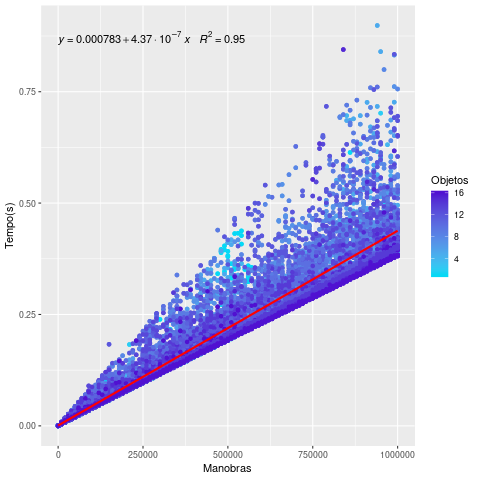
\includegraphics[width=0.5\textwidth]{normal-data-gg.png}
\caption{Tempo total do algoritmo com espalhamento normal.\label{fig:normal-data-total}}
\end{figure}

\begin{figure}[htbp]
\centering
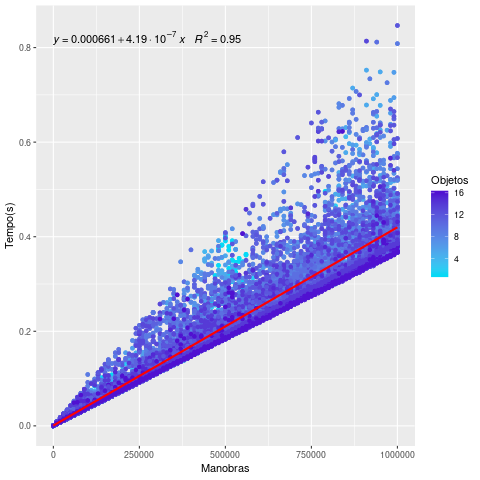
\includegraphics[width=0.5\textwidth]{perfect-data-gg.png}
\caption{Tempo total do algoritmo com espalhamento perfeito.\label{fig:perfect-data-total}}
\end{figure}

É possível ver que a complexidade calculada foi comprovada, os gráficos mostram uma complexidade linear.

Pode-se notar que o espalhamento perfeito possui alguns fatores na equação linear que demonstram ser um pouco mais rápido, porém esse valor é muito pequeno. Isso demonstra que a tabela de dispersão normal possivelmente está na média colidindo muito pouco.

Ou seja por causa da limitação de objetos no mapa o algoritmo com espalhamento perfeito e espalhamento normal se diferenciam por uma constante.

\bigskip
Veja uma simples média de tempo dos dados com 100000 manobras.
\begin{center}
\begin{tabular}{|c|c|}
\hline
Espalhamento normal & Espalhamento perfeito\\
\hline
0.04566633s & 0.04402262s\\
\hline
\end{tabular}

\end{center}

É possível notar que o espalhamento perfeito na média para muitas manobras possui execução mais rápida.

Será analisado se isso se mantém para quantidades menores de manobra, especificamente 1000 manobras.

\begin{center}
\begin{tabular}{|c|c|}
\hline
Espalhamento normal & Espalhamento perfeito\\
\hline
0.00013292s & 0.00012228s\\
\hline
\end{tabular}

\end{center}

Pelo visto o espalhamento perfeito esta conseguindo tempos menores, então só falta uma visão geral dessas médias e intervalo de confiança das mesmas. Observe na figura \ref{fig:means-data}.

\begin{figure}[htbp]
\centering
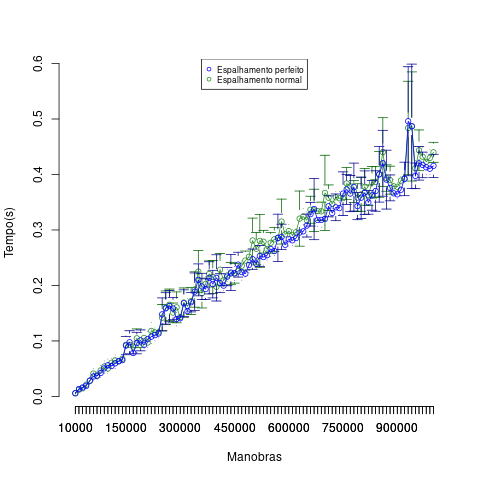
\includegraphics[width=0.52\textwidth]{means-data.png}
\caption{Média dos tempos dos algoritmos.\label{fig:means-data}}
\end{figure}


O gráfico mostra que o programa com espalhamento perfeito na maioria das vezes tem uma média de tempo menor que o programa com espalhamento normal.

Para um conjunto menor de manobras fica evidente que uma domina a outra por uma constante. (Figura \ref{fig:means-obj-100-data})



\begin{figure}[htbp]
\centering
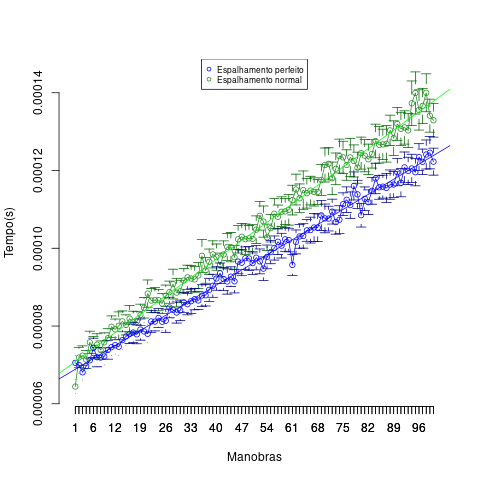
\includegraphics[width=0.33\textwidth]{means-obj-100-data.png}
\caption{Média dos tempos com pequena quantidade de manobras.\label{fig:means-obj-100-data}}
\end{figure}


\subsection{Objetos}
\label{sec:org98e9be4}
Com a análise do comportamento do custo da função com o aumento do número de manobras só falta analisar o aumento do tempo da função com base no aumento do número de objetos. (Figura \ref{fig:means-data-total})

\begin{figure}[htbp]
\centering
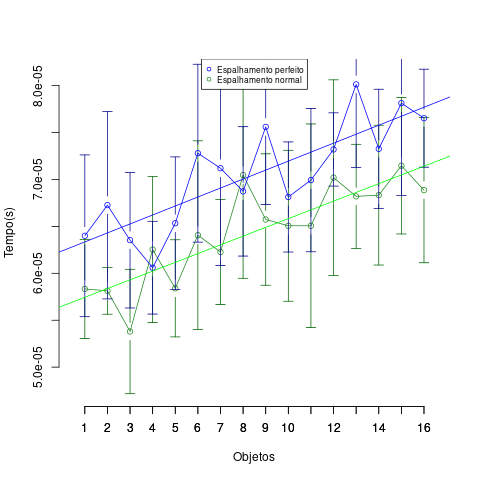
\includegraphics[width=0.43\textwidth]{means-obj-data.png}
\caption{Média dos tempos de acordo com a quantidade de objetos, 1 manobra.\label{fig:means-data-total}}
\end{figure}

\begin{figure}[H]
\centering
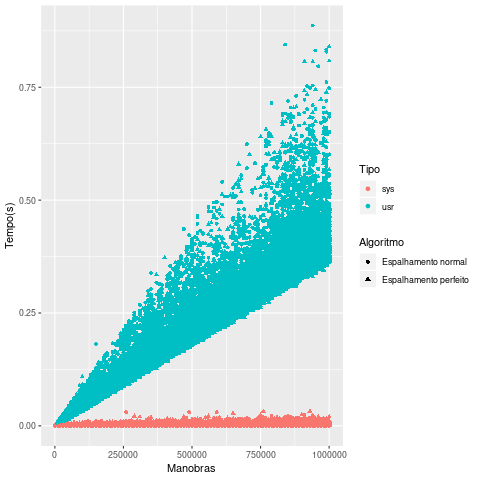
\includegraphics[width=0.6\textwidth,height=6cm]{usr-sys-data-gg.png}
\caption{Tempo de usuário e sistema.\label{fig:usr-sys-data}}
\end{figure}

A primeira coisa que o gráfico mostra é que para um certo valor pequeno de manobras, que no caso é 1, o algoritmo com espalhamento normal ainda consegue ser mais rápido que o algoritmo com espalhamento perfeito. 

E a outra informação que pode ser obtida é que o crescimento do tempo de acordo com o crescimento da quantidade de objetos parece ser um crescimento linear para ambos algoritmos. Como a complexidade do algoritmo com espalhamento normal na iniciação do estacionamento é \(O(Objs^2)\) \eqref{eq:parkinginit} o gráfico deveria apresentar esse comportamento, mas por causa do limite de objetos se torna inviável fazer uma regressão polinomial, ou seja a complexidade assintótica \(O(1)\) também está comprovada.

\subsection{Tempo de sistema e usuário}
\label{sec:orgffb0028}
O tempo de usuário é o tempo associado ao tempo de processamento no modo de usuário ou fora do núcleo do sistema \cite{kernel}. Ou seja o tempo de usuário contém o tempo processando o código do programa e das bibliotecas que o compõe, tempos de entrada e saída por exemplo não são contabilizados.
Já o tempo de sistema é o tempo gasto no núcleo dentro do processo ou simplesmente o tempo gasto no modo sistema no processo, já que o usuário não pode fazer todo tipo de operação possível com os recursos de um computador o núcleo do sistema é quem faz o intermédio para gerenciar as chamadas de operações privilegiadas do usuário (exemplo I/O).

Um exemplo é se o algoritmo for recursivo as computações locais serão somadas no tempo de usuário e a chamada a função de recursão guardara todas variáveis locais atuais na pilha do sistema e quem gerencia isso é o núcleo do sistema logo somara o tempo dessa operação no tempo de sistema. Visto que não há muitas chamadas ao sistema e também principalmente não há nenhum algoritmo recursivo o tempo no modo sistema se manteve baixo como é mostrado na figura \ref{fig:usr-sys-data}.

\section{Apêndice}
\label{sec:orgf0305e6}
\subsection{Shell script para coleta de dados}
\label{sec:org3c7ca7c}
Algoritmo \textbf{data-catch}.
\begin{lstlisting}
data-catch <initial config file> <maneuvers> <execution times> <initial value> <step> <final value>
\end{lstlisting}

Foi utilizado o gerador de configurações iniciais para fazer mapas de 1 a 16 objetos. E a cada configuração criada era observado se o mapa conseguiria suportar um movimento de "vai e volta" de um carro em especifico, se conseguisse preserva o arquivo, se não utiliza o gerador para a quantidade de objetos em especifico.

\begin{lstlisting}
for ((i=1;i<=16;i++));do ./generator -n $i -o objs"$i".txt; done
\end{lstlisting}

Com os estacionamentos criados e a manobra sendo valida para todos eles então é so começar a guardar os dados com o auxiliar que foi criado acima.

\begin{lstlisting}
times=20
for ((i=1;i<=16;i++)); do ./data-catch objs"$i".txt manobras.txt $times 10000 10000 1000000; done
for ((i=1;i<=16;i++)); do ./data-catch objs"$i".txt manobras.txt $times 1 1 100; done
\end{lstlisting}

\subsection{Gerador de configurações iniciais}
\label{sec:org3a24eb2}
Foi feito um gerador de configurações iniciais. A sua utilização pode ser vista a seguir:
\begin{verbatim}
generator -n <number of objects> & -o <output file>
\end{verbatim}

\bibliographystyle{plain}
\bibliography{doc}
\end{document}
